% Use only LaTeX2e, calling the article.cls class and 12-point type.

\documentclass[10pt,a4paper]{mjcs}
% Use times if you have the font installed; otherwise, comment out the
% following line.

\usepackage{times}
\usepackage{graphicx}
\usepackage{multirow}
\usepackage[figurename=Fig.]{caption}
\captionsetup[figure]{labelsep=period}
\captionsetup[table]{labelsep=period}

% The preamble here sets up a lot of new/revised commands and
% environments.  It's annoying, but please do *not* try to strip these
% out into a separate .sty file (which could lead to the loss of some
% information when we convert the file to other formats).  Instead, keep
% them in the preamble of your main LaTeX source file.


% The following parameters seem to provide a reasonable page setup.

\topmargin -1.5cm
\oddsidemargin 0.2cm
\textwidth 16cm
\textheight 24cm
%\footskip 1.0cm


\setlength{\parindent}{0em}
\setlength{\parskip}{0.7em}


%The next command sets up an environment for the abstract to your paper.

\newenvironment{mjcsabstract}{%
\begin{flushleft}
\textbf{\textit{ABSTRACT}}
\end{flushleft}

\it}


% If your reference list includes text notes as well as references,
% include the following line; otherwise, comment it out.

% Include your paper's title here

\title{Simplistic approach for Computing Disparity map}


% Place the author information here.  Please hand-code the contact
% information and notecalls; do *not* use \footnote commands.  Let the
% author contact information appear immediately below the author names
% as shown.  We would also prefer that you don't change the type-size
% settings shown here.

\author
{Chitra Suresh $^{1\ast}$ Kushal R. Tuckley \\
\\
\normalsize{$^{1\ast}$,RamRao Adik Institute of Technology,Nerul,NaviMumbai-400706}\\
\normalsize { Adjunct Professor, IIT Bombay ,Chairman and Director R$\&$D, \textbf{AGV} Systems Pvt Ltd.Mumbai-400076}\\
%\normalsize{$^{2}$Another Unknown Address, Palookaville, ST 99999, UBCD}\\
%\\
\normalsize{$^\ast$E-mail:chitra.suresh@rait.ac.in }
\normalsize{E-mail:kushal@ee.iitb.ac.in }
}

% Include the date command, but leave its argument blank.

\date{}


\usepackage{fancyhdr}

\pagestyle{fancy}
\fancyhf{}
\renewcommand{\headrulewidth}{0pt}
\rhead{Simplistic approach for Computing Disparity map}
%\lhead{Authors}



%%%%%%%%%%%%%%%%% END OF PREAMBLE %%%%%%%%%%%%%%%%



\begin{document}

% Double-space the manuscript.

\baselineskip12pt

% Make the title.

\maketitle




%%{Ms.Chitra Suresh ,$^{1\ast}$ Dr. Kushal R. Tuckley ,$^{1}$ %Joe Scientist$^{2}$\\
%%\\
%%\normalsize{$^{1}$D.Y.Patil' RAIT,Dr.D.Y.Patil Vidyanagar,Setor-7,Nerul,NaviMumbai-400706}\\
%%\normalsize{Adjunct Professor, IIT Bombay ,Chairman and Director R&D, \textbf{AGV} Systems Pvt Ltd.Mumbai-400076}\\
%%%\normalsize{$^{2}$Another Unknown Address, Palookaville, ST 99999, UBCD}\\
%%%\\
%%\normalsize{$^\ast$E-mail:  jsmith@wherever.edu.}
%%\normalsize{$^\ast$E-mail:  jsmith@wherever.edu.}
%}
%
%% Include the date command, but leave its argument blank.
%
%\date{}
%
%
%\usepackage{fancyhdr}
%
%\pagestyle{fancy}
%
%
%
%
%
%\fancyhf{}
%\renewcommand{\headrulewidth}{0pt}
%\rhead{Guidelines for Malaysian Journal of Computer Science}
%%\lhead{Authors}
%
%
%
%%%%%%%%%%%%%%%%%% END OF PREAMBLE %%%%%%%%%%%%%%%%
%
%
%
%\begin{document}
%
%% Double-space the manuscript.
%
%\baselineskip12pt
%
%% Make the title.
%\maketitle
%


% Place your abstract within the special {sciabstract} environment.

\begin{mjcsabstract}
In this paper, a simple technique called 'minimum index method' is presented for the computation of disparity map. The Semi Global Block Method is a popular method available in most of the standard computation tools in  Matlab. The paper has compared the performance of Semi Global Block Method with the proposed method. The  standard method used is the in-build function 'Disparity Map' from the computer vision tool box in MATLAB. In the minimum index method, The Sum Absolute Difference (SAD)is used to find disparity. The right image in input stereo image is shifted column wise depending on the size of disparity. The size of the disparity varies one to sixteen. In the depth map by  minimum index method, the minimum disparity occurs in Sum Absolute Difference(SAD) matrix. The simulated results shows that in minimum index method objects in depth map are better recognizable than Semi Global Block method. The mean square error is less in minimum index method than Semi Global Block method.
\end{mjcsabstract}

\keywords{Stereo image, Depth Map and Sum Absolute Difference (SAD)}


\section{Introduction}

The disparity map or depth map is to measure horizontal pixel distance for each pixel coordinate, the horizontal  distance between two matching pixels is disparity. The amount of disparity depends on the depth. The depth is difference in distance between two objects and distance to the point of fixation which is known as parallax effect. The same principle is used to find disparities for stereoscopic images.
\newline The stereoscopic images or stereo pair consists of two images of the same scene taken slightly horizontally with separated points from the left view and the right view. The parallax effect also presents stereoscopic images in such a way that objects near the camera will represent more to the right in the left image and more to the left in the right image. The horizontal displacement of an object in the left and right view depends on the distance from the object to the camera viewpoints.
\newline There are various methods to find Disparity map or Depth map. The various methods are Area-based, Feature- based and Global-based methods. The Area and feature based methods are based on intensity profile. The Global methods are based on Bayesian approach that finds disparity as an energy minimization problem.
Standard methods of computing disparity is as follows:
Method and brief description with reference.
\newline [1]  The method used in "Adaptive support -weight approach for correspondence search" is area-based local method to generate depth map or disparity map. The proposed method is based on Gestalt grouping in which support weight is based on similarity and proximity and is proportional to the strength of the grouping. In this method these two values are expressed as a single value in an integrated manner. The group of similarity is calculated by means of Euclidean distance whereas group of proximity is calculated by means of Laplacian Kernel. The weight adoptive method computationally takes longer time than other methods.
Method and brief description with reference.
\newline [2]  The method used in "A New Approach for Disparity Map Estimation from stereo Image Sequences using Hybrid Segmentation Algorithm" is feature-based local method to generate Depth map or Disparity map. The estimation of Disparity map is by using K-mean square algorithm and hybrid segmentation algorithm. The K means clustering algorithm is used to group the objects based on some criteria; K is a positive integer. The criteria for grouping is by minimizing the distance between data and cluster centroid. Initial set of K, virtual points in the dataspace is randomly selected and every point of data set is assigned the nearest centroid. The position of centroid is updated by means of the data points assigned to the cluster. The algorithm is stopped when the minimum shift is below threshold. The segmentation algorithm extracts feature by Scale Invariant Feature Transform (SIFT) and Sum of Absolute Difference(SAD).The proposed algorithm is complex and  the computation time is higher.
 \newline [3] The method used in "A Comparative Study of Energy Minimization Methods for Markov Random Fields" is global based method to generate Depth map or Disparity map. The method used is energy minimization problem on rectangular grid of pixels where energy is expressed as data term and smoothness term. The method used is complex and the computation time is higher.
However, all these method do not produce good results or work well for specific types of images
We suggest a simple method ensuring a good performance for different kinds of images.
\newline Some application of Depth maps for robot application for navigation purpose and for object recognition to separate occluded image components. Another important scientific application of Depth map or Disparity map is to extract information from aerial surveys and for calculation of contour maps.
\newline The  organization of paper is as follows ,the methods used for comparative study is explained in section 2, The results for comparative study is shown in section 3 , Discussion for proposed method in section 4 and the conclusion of the paper in section 5.




\section{METHODS USED FOR COMPARATIVE STUDY }
The Semi Global Block  method and Minimum Index method are used to generate Depth map or Disparity map.
The input image is stereo images.\newline The block diagram shown below indicates methods used for comparative study.
\begin{figure}[htbp]
\centering
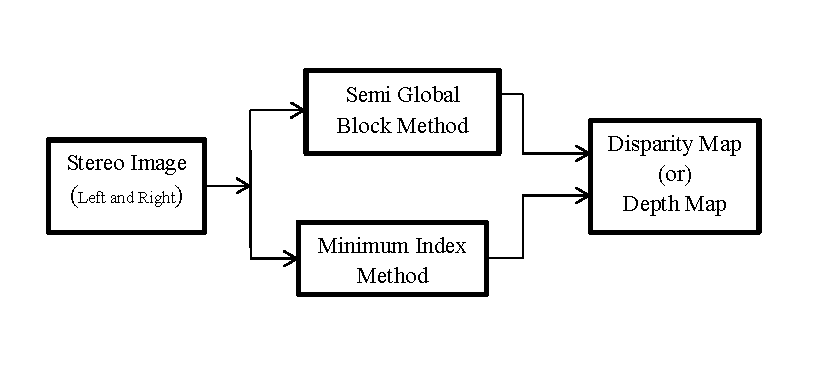
\includegraphics{compa.eps}
\caption{\textbf{Disparity Map Comparison Approach .}}
\label{mjcs}
\end{figure}
\subsection{Image Rectification for stereo Images}


\begin{figure}[htbp]
\centering
\includegraphics{doc3.eps}
\caption{\textbf{Conceptual diagram for image rectification[6]}}
\label{mjcs}
\end{figure}
The images taken from two cameras aligned horizontally using linear transformations which  rotate, translate and skew the camera images. The image rectification is method that  produce epipolar lines of two camera images aligned horizontally.After image rectification has been carried out,two projected points in epipolar lines becomes parallel and aligned horizontally\newline
A two dimensional search becomes one dimensional search along horizontal lines after image rectification.It becomes easy to analyze stereo images.
\newline The concept  of image rectification is shown in Fig.2. The original camera image planes are drawn with solid borders and the rectified image planes are drawn with dashed borders.[6] The epipolar lines are also drawn from the projected points p and p' to epipoles e and e'\newline The  image referred as a left image corresponding to camera 1 is specified in 2-D grayscale. The  image referred as  a right image  corresponding to camera 2 is also specified in 2-D gray scale.The Input images left and right must be real,finite and non sparse.They must be of the same class.
\subsection{Semi Global Block Method}
In Semi Global Block method [4],The Disparity map is generated using the computer vision tool box function  of MATLAB. The  function used from computer vision tool box is 'Disparity map'. The algorithm used to estimate disparity in Semi Global Block  method is Semi Global Block matching algorithm. The sum of absolute difference is used to compare each block of pixel in stereo image and Semi  Global  Block matching algorithm enforces similar disparity to neighbouring blocks.
\newline The Semi Global Block matching algorithm measures the contrast of stereo image by using sobel filter. The Semi Global Block matching algorithm finds the disparity for each pixel in the left stereo image.
\newline In  Semi Global Block method, the range of  disparity is a two element vector and must be in the format of [Min disparity, Max disparity]. Both elements in disparity range vector must be integers and can be negative. Min disparity and  Max disparity must be in the range [-imagewidth, imagewidth]. The difference between Max disparity and Min disparity must be divisible by 16.
\subsection{ Minimum Index Method}
The Sum Of Absolute Difference (SAD) is used in this method. The disparity or label is fixed to 16.The right image is shifted  to column wise 1to16,which depends on the size of disparity, then disparity is found where minimum disparity occurs.
\subsubsection{Pseudo code for Minimum Index Method}
The Pseudo code for Minimum Index Method is shown below:
\begin{enumerate}
  \item Left Image = LI of dimension (M X N) = the elements are indicated by =LI(i,j)
  \item Right Images= RI of dimension (M X N) = the elements are indicated by =RI(i,j)
  \item for    i=1:M
  \item for j=16:N     \% Shift of 16 is used to avoid edge-overflow
  \item E1(i,j)=abs\{LI(i,j)-RI(i-1,j)\}....... E16(i,j)=abs\{LI(i,j)-RI(i-16,j)\}
  \newline \% E(k) is a vector of 16 elements corresponding to each pixel values.\newline
        \%Difference in pixel value is computed for all 16 steps

  \item D(i,j)= min{(E1(i,j),E2(i,j),E3(i,j)........E16(i,j))}\newline
                   \% The disparity value is decided where, minimum difference in pixel values is observed.\newline
  \% In other words,if $E(5)_{i,j}$ is the minimum value of$ E(k)_{i,j}$ then D(i,j)= 5.
  \item end
  \item end
\end{enumerate}

\section{SIMULATED RESULTS}

The  stereo images for testing are from  data sets 2014 of Middlebury computer vision website (vision.middlebury.edu).\newline
Baby, Bowling, Cloth and Pot are considered as test stereo images and these images have ground truth.





\begin{table}[htbp]
\caption{Dimension and size of Input stereo image and reference (ground truth) image.}
\begin{center}
\begin{tabular}{|l|l|l|l|l|}
\hline
Image Type & Stereo Left Image &Stereo Right Image &Ground Truth Left & Ground Truth Right \\
\hline
Baby& 437X370
(230kb)
 & 437X370
(229kb)
 & 437X370
(18.5kb)
&437X370
(18.7kb)
 \\
\hline
Blowing & 443X370
(235kb)
 & 443X370
(230kb)
 & 443X370
(21.2kb)
 & 443X370
(21.4kb)
\\
\hline
Cloth& 433X370
(315kb)
 &433X370
(320kb)
  &433X370
(19.8kb)
 &433X370
(20.6kb)
 \\
\hline
Pot & 437X370
(189kb)
 & 437X370
(188kb)
 & 437X370
(20kb)
 &437X370
(20.5kb)
 \\

\hline
\end{tabular}
\end{center}
\label{parameter_values}
\end{table}

\begin{table}[htbp]
\caption{Mean Square Error for both methods for test images.}
\begin{center}
\begin{tabular}{|l|l|l|l|}
\hline
Stereo Image & Minimum Index Method(MSE)& Standard Method(MSE)  \\
\hline
Baby & 2150 & 16950  \\
\hline
Bowling & 3074 & 19526  \\
\hline
Cloth & 2177& 20137  \\
\hline
Pot & 3143 & 17229  \\

\hline
\end{tabular}
\end{center}
\label{parameter_values}
\end{table}

\begin{table}[htbp]
\caption{Dimension  and Run time of Depth Map by Minimum Index Method.}
\begin{center}
\begin{tabular}{|l|l|l|l|}
\hline
Test Image & Size of Depth Map & Run time  \\
\hline
Baby & 611 X 465(93.4KB) & 10.5sec   \\
\hline
Blowing  & 617 X 465(93.5KB) & 1.4 sec  \\
\hline
Cloth  & 607 X 465(110KB) & 1.68sec \\
\hline
Pot & 611 X 465(76.8KB)  & 1.68sec  \\

\hline
\end{tabular}
\end{center}
\label{parameter_values}
\end{table}

\begin{table}[htbp]
\caption{Dimension and Run time of Depth Map by Semi Global Block Method.}
\begin{center}
\begin{tabular}{|l|l|l|l|}
\hline
Test Image & Size of Depth Map & Run time  \\
\hline
Baby & 611X465(20.6KB) & 0.82 sec  \\
\hline
Blowing  & 617 X 465(15.8KB) & 0.7sec  \\
\hline
Cloth  & 607 X 465(8.5KB) & 0.73sec  \\
\hline
Pot & 611 X 465(13.3KB)  &  1.02sec \\

\hline
\end{tabular}
\end{center}
\label{parameter_values}
\end{table}



\begin{figure}[htbp]
\centering
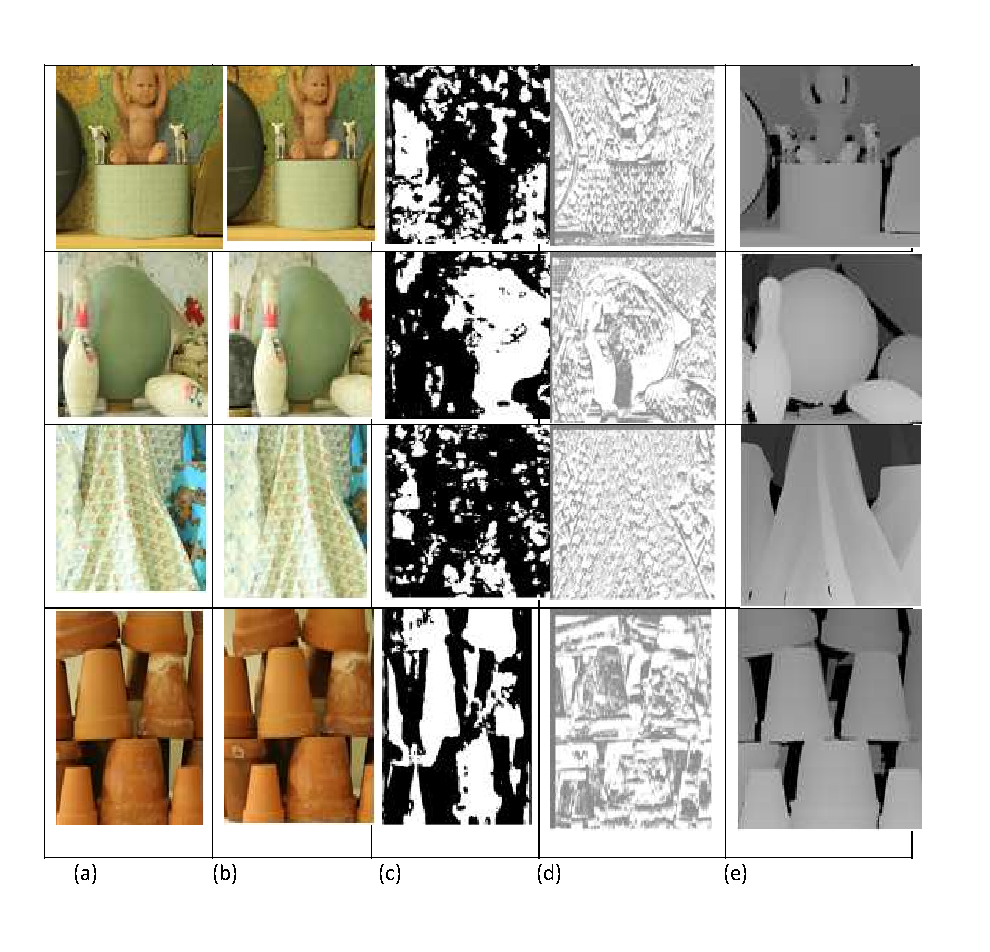
\includegraphics{DM_MA_MI.eps}
\caption{\textbf{Stereo input images and Depth maps(a) Left Image (b) Right Image  (c) Depth map by Semi Global Block method (d) Depth map by Minimum  Index Method (e) Ground truth.}}
\label{mjcs}
\end{figure}

\section{DISCUSSION}The performance comparison was done subjectively by human perception as well as by computation of mean squared error with the ground reality image. The Depth map for different test stereo image by both methods (Semi Global Method and Minimum Index method) are shown in Fig.3.\newline Details of test stereo images and reference (ground truth) images are shown in table 1\newline We have found that the proposed method for Baby and Bowling test stereo image gives 7 times, Cloth test stereo image 10 times and Pot test stereo image 6 times less Mean Square Error(MSE) as compared to Semi Global Methods which is shown in table 2.\newline The run time for both methods computed on a  system Intel(R) Core(TM) i5-4200M CPU @2.5GHz using MATLAB Version 15.The size of depth map obtained by Minimum Index Method and  Semi Global Block  method  for different test stereo images with run time shown in table 3 $\&$table 4 respectively.
\section{CONCLUSION} In this paper, we have proposed a new method to generate Depth map using Sum Of Absolute Difference (SAD) for stereo images. The Depth map by proposed minimum index method is compared with Semi Global Block method.\newline The Semi Global Block method recovers Depth map using MATLAB in build function 'Disparity Map' from computer vision tool box.\newline The proposed method shows much better agreement with the 'ground truth image', when compared with  'Semi Global Block'  method available as a standard utility in MatLab. It takes marginally more computation time across different types of images that, objects  in Depth map  as comparable to ground truth image whereas in  Semi Global Block method it is difficult to identify  objects in Depth map. \newline The runtime for both methods are almost same but Mean Square Error (MSE) is less in Minimum Index method than Semi Global Block method for all test stereo images. With this performance Minimum Index method has can be used as  generic method.

\subsection{FUTURE WORK}The Initial Depth Map generated by Minimum Index Method and  Semi Global Block  method  can be improved by using  optimization algorithm like Graph cut and Belief Propagation.


\section*{Copyright}
It is a condition of publication that manuscripts submitted to the journal have not been published, accepted for publication, nor simultaneously submitted for publication elsewhere. By submitting a manuscript, the author(s) agree that copyright for the article is transferred to the publisher, if and when the manuscript is accepted for publication.

\begin{thebibliography}{10}

\bibitem{01}
L. kuk-Jin Yoon, In Sokweon , {''Adaptive support -weight approach for correspondence search''}.IEEE Transactions on pattern analysis and machine Intelligence, Vol. 28,no.4,April 2006,pp 650-651.

\bibitem{02}
Patrik Kamencay,Martina Zachariasova,Martin Brezman,Roman Jarina,Robert Hudec,Miroslav Benco ,Slavomir Matuska, {''A New Approach for Disparity Map Estimation from stereo Image Sequences using Hybrid Segmentation Algorithm''}, International Journal of Modern  Engineering Research,Vol.2,Issue 5,Sep-Oct 2012 ,pp3201-3206

\bibitem{03}
R. Szeliski, R. Zabih, D. Scharstein, O. Veksler, V. Kolmogorov, A. Agarwala, M. F. Tappen and C. Rother,., {''A Comparative Study of Energy Minimization Methods for Markov Random Fiel''}, IEEE Trans. Pattern Anal. Mach. Intell., vol. 6, no. 30, (2008), pp. 1068-10
\bibitem{04}
Http://in.mathworks.com/help/vision/ref/disparity.html
\bibitem{05}
Brad Hiebert-Treuer,Sarri Al Nashashibi and Daniel Scharstein ,Middlebury stereo vision pages,http:// Vision.middlebury.edu.
\bibitem{06}M. Z. Brown, D. Burschka, and G. D. Hager, "Advances in computational stereo," IEEE Transactions on Pattern Analysis and Machine Intelligence, vol. 25, no. 8, pp. 993-1008, 2003.

\bibitem{07}S. B. Kang and R. Szeliski, "Extracting View-Dependent Depth Maps from a Collection of Images", Int'l J. Computer Vision, vol. 2, no. 58, (2004), pp. 139-163
\bibitem{08}G.Gerig,www.Sci.Utah.edu/gerig/CS6320-S2013/�../CS6320-cv-F2012-Rectification.pdf

\bibitem{09} https://www.CSE.Unr.edu/bebis/CS791E/Notes/EpipolarGeonetry.pdf
\bibitem{10}Colin Doutre and Panos Nasiopoulos," A Stereo matching Datacost Robust to Blurring", IEEE 17th International conference on Image Processing, September 26-29, 2010, Hong Kong
\bibitem{11}W. D. Hu, K. Zhang, L. F. Sun, J. Y. Li, Y. J. Li and S. Q. Yang, "Virtual Support Window for Adaptive-weight Stereo Matching",  IEEE Visual Communications and Image Processing (VCIP), (2011) November 6-9, pp. 1-4, Tainan, Taiwan.

\bibitem{12}Komal D.Bhavsar, Virendra Singh," Analysis of Disparity Map for stereo Matching Algorithm", International Journal for scientific Research $\&$ Development,Vol.1,IIsue 11,2014,ISSN(online):2320613

\bibitem{13}Y. Boykov, O. Veksler and R. Zabih,"Markov Random Fields with Efficient Approximations, Proc. IEEE Int. Conf. Pattern Analysis and Machine Intelligence, (1998) June 23-25, pp. 648-655, Santa Barbara, CA, USA.

\bibitem{14}Somon Hermann,Reinhard Klette" The Naked Truth about cost functions for stereo matching", http://www.mi.auckland.ac.nz/EISATS
\bibitem{15}LiCheng,TerryCaellu ,"Bayesian Stereo matching" ,Computer vision and Image understanding,
http://www.elsevier.com/locate/eviu


\bibitem{16}R. Klette and S. Morales, "Prediction Error Evaluation of Various Stereo Matching Algorithms on Long Stereo Sequences," 2009.
\bibitem{17}David A. Forsyth and Jean Ponce, Computer Vision: A Modern Approach, US ed.: Prentice Hall, 2002.
\bibitem{18}R. Klette and S. Morales, "Prediction Error Evaluation of Various Stereo Matching Algorithms on Long Stereo Sequences," 2009.
\bibitem{19}Olga Veksler,"Efficient graph-based energy minimization methods in computer vision," 1999.


\end{thebibliography}
\section{BIOGRAPHY}

\begin{figure}[htbp]
\centering
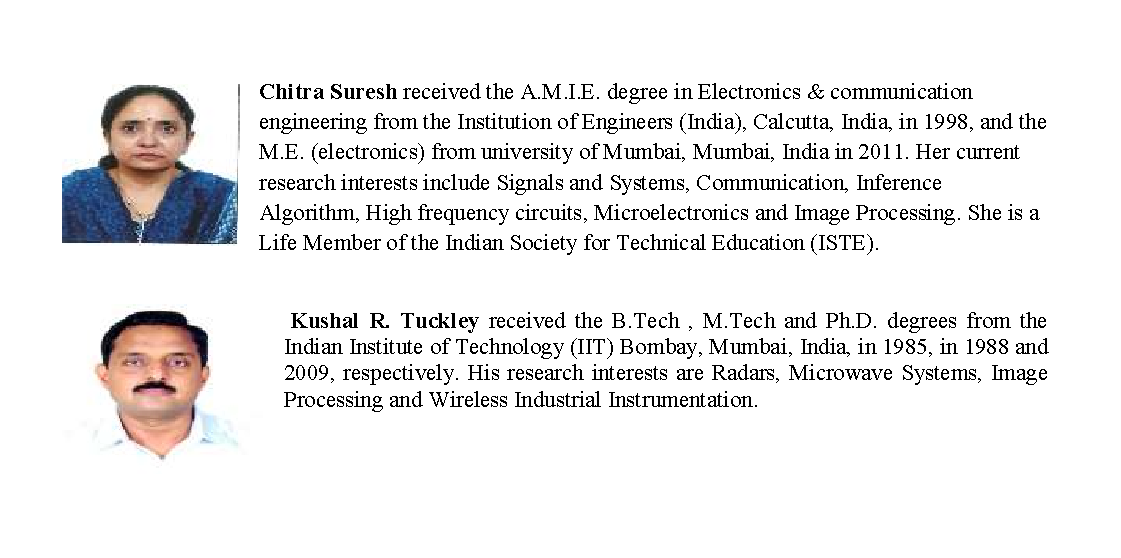
\includegraphics{bio.eps}
\label{mjcs}
\end{figure}


\end{document}



















